\begin{figure*}
  \centering
  \begin{tabular}{c c c c c c c}
    \begin{sideways}\bf \small\quad\quad $\detroi$\end{sideways}&
    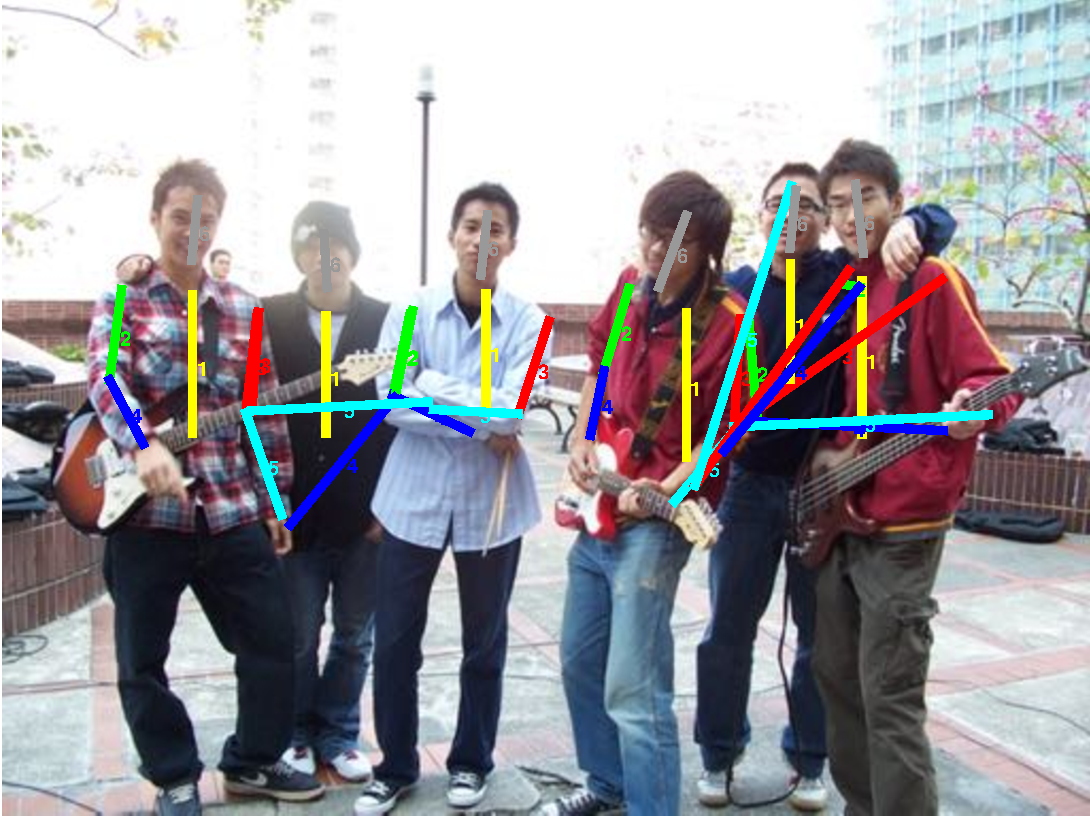
\includegraphics[height=0.145\linewidth]{imgidx_0112_sticks_unary_waf.pdf}&
    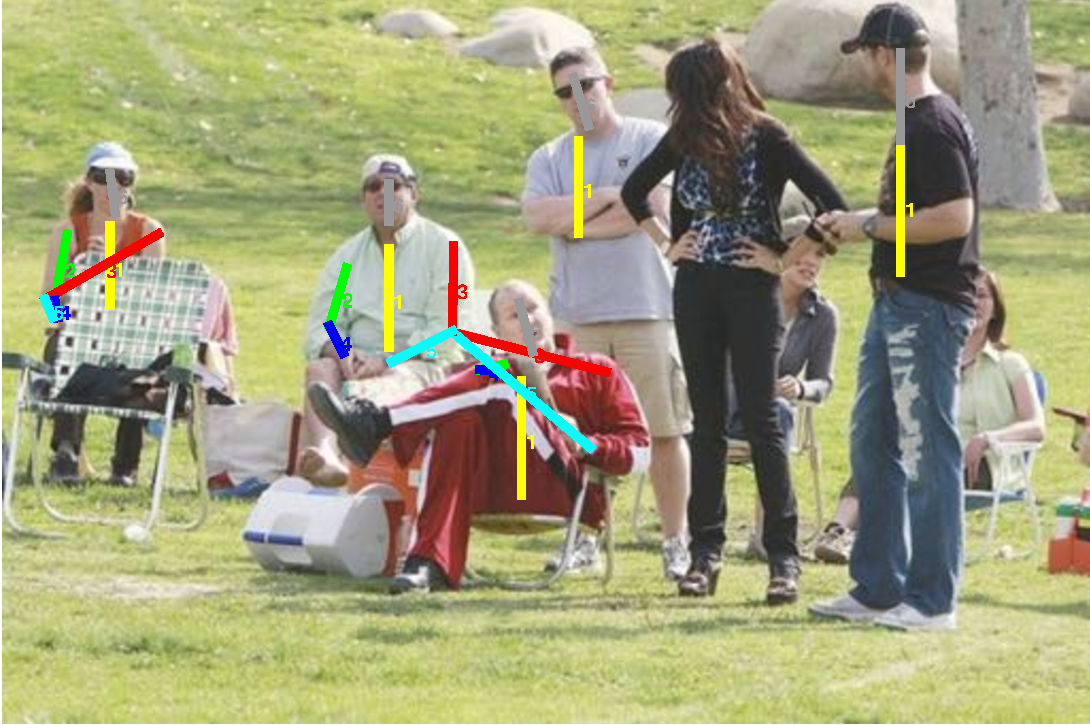
\includegraphics[height=0.145\linewidth]{imgidx_0028_sticks_unary_waf.pdf}&
    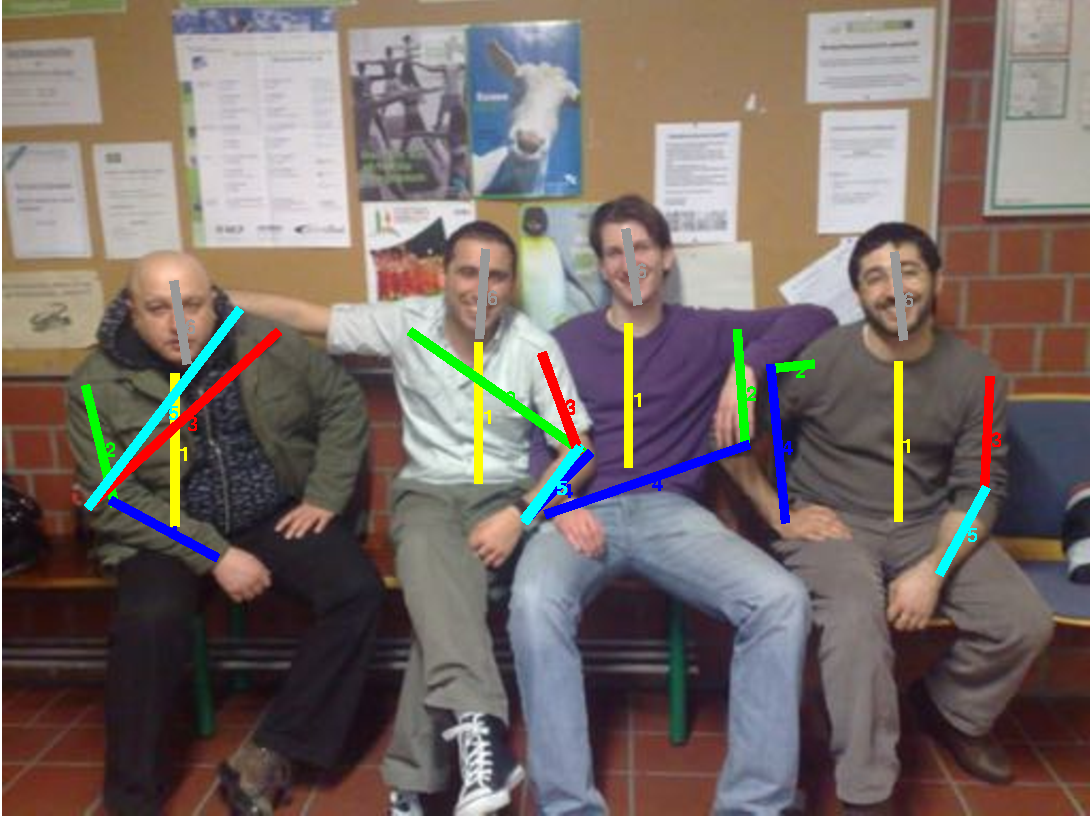
\includegraphics[height=0.145\linewidth]{imgidx_0129_sticks_unary_waf.pdf}& 
    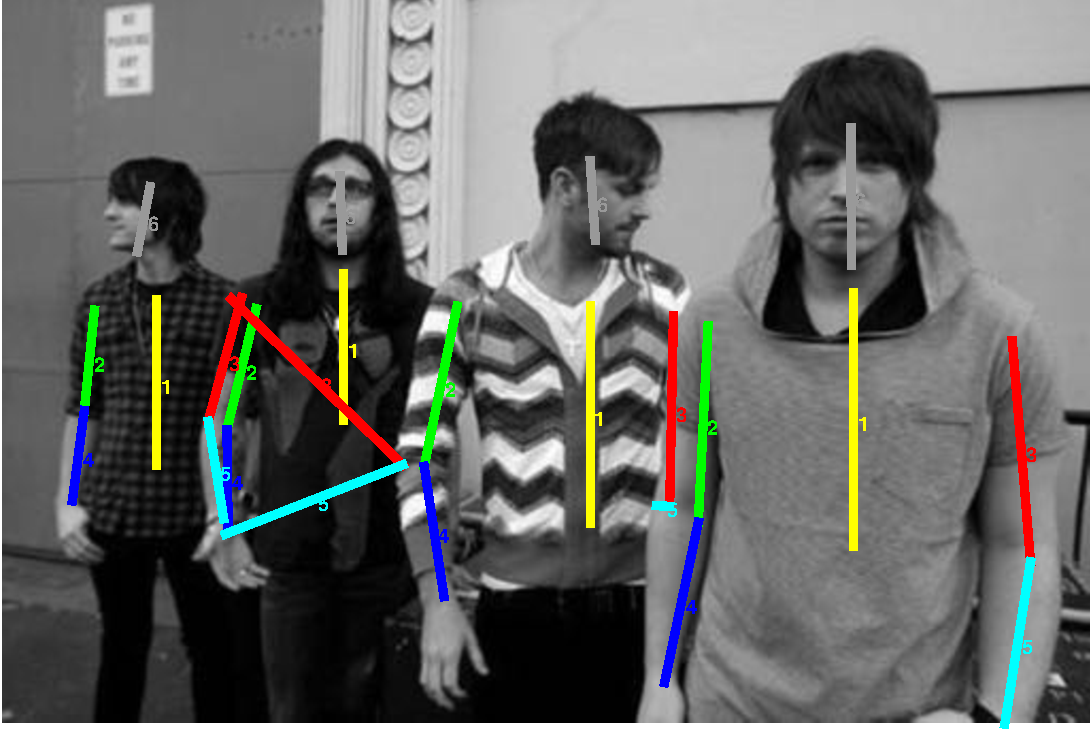
\includegraphics[height=0.145\linewidth]{imgidx_0078_sticks_unary_waf.pdf}& % 58
    %\includegraphics[height=0.145\linewidth]{imgidx_0020_sticks_unary_waf.pdf}& % 66 
    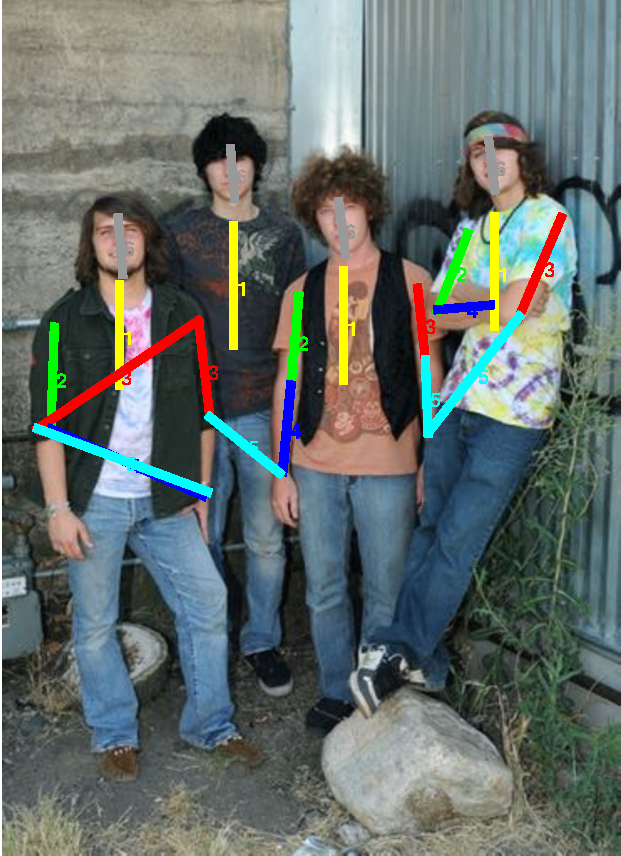
\includegraphics[height=0.145\linewidth]{imgidx_0139_sticks_unary_waf.pdf}\\ 
    \begin{sideways}\bf \small\quad $\deepcut~\multb$\end{sideways}&
    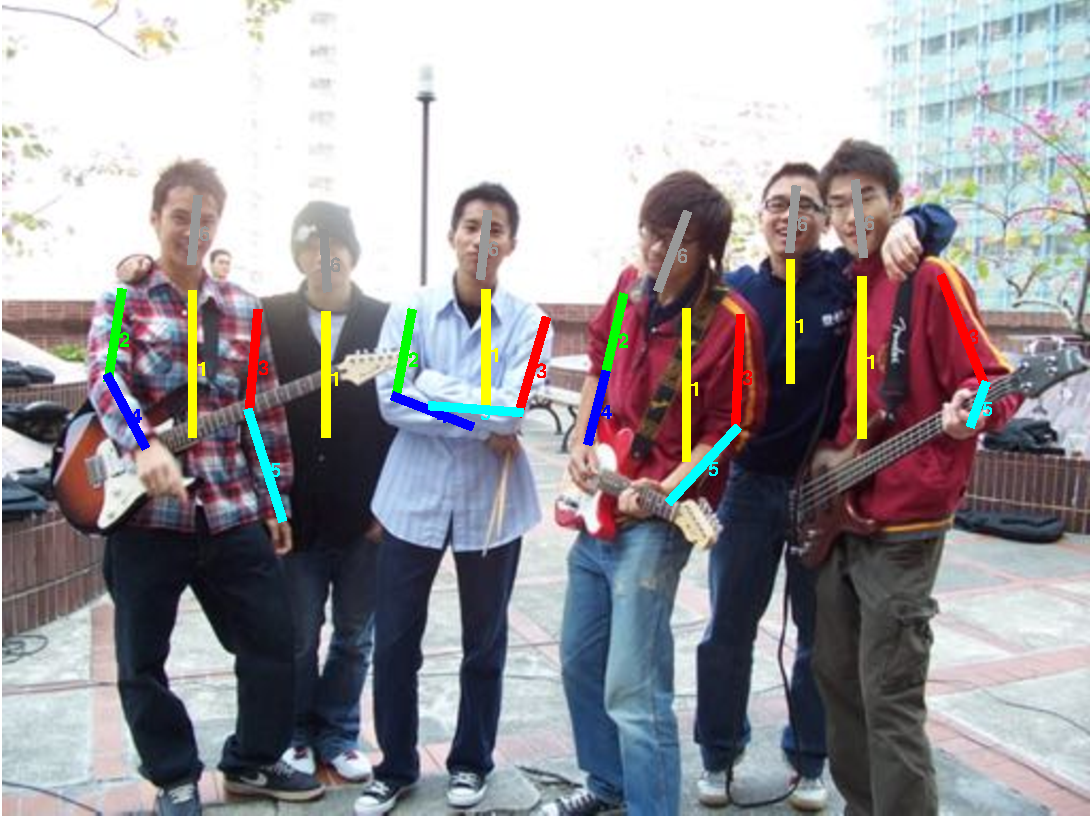
\includegraphics[height=0.145\linewidth]{imgidx_0112_sticks_waf.pdf}&
    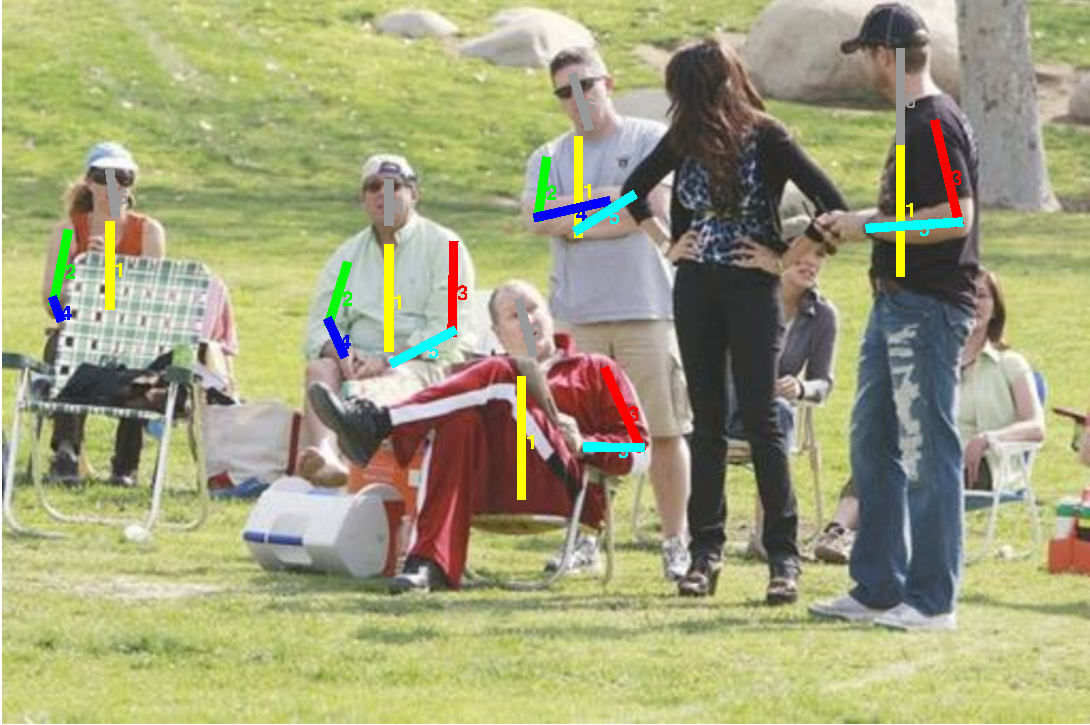
\includegraphics[height=0.145\linewidth]{imgidx_0028_sticks_waf.pdf}&
    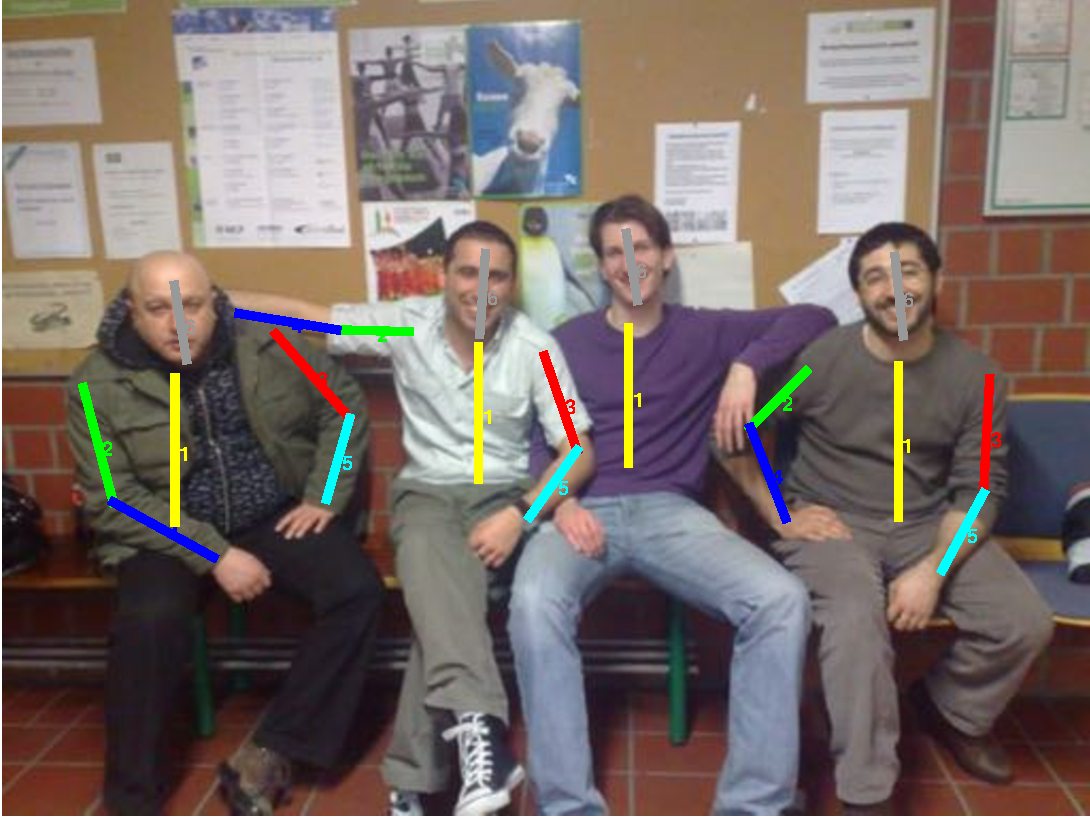
\includegraphics[height=0.145\linewidth]{imgidx_0129_sticks_waf.pdf}&
    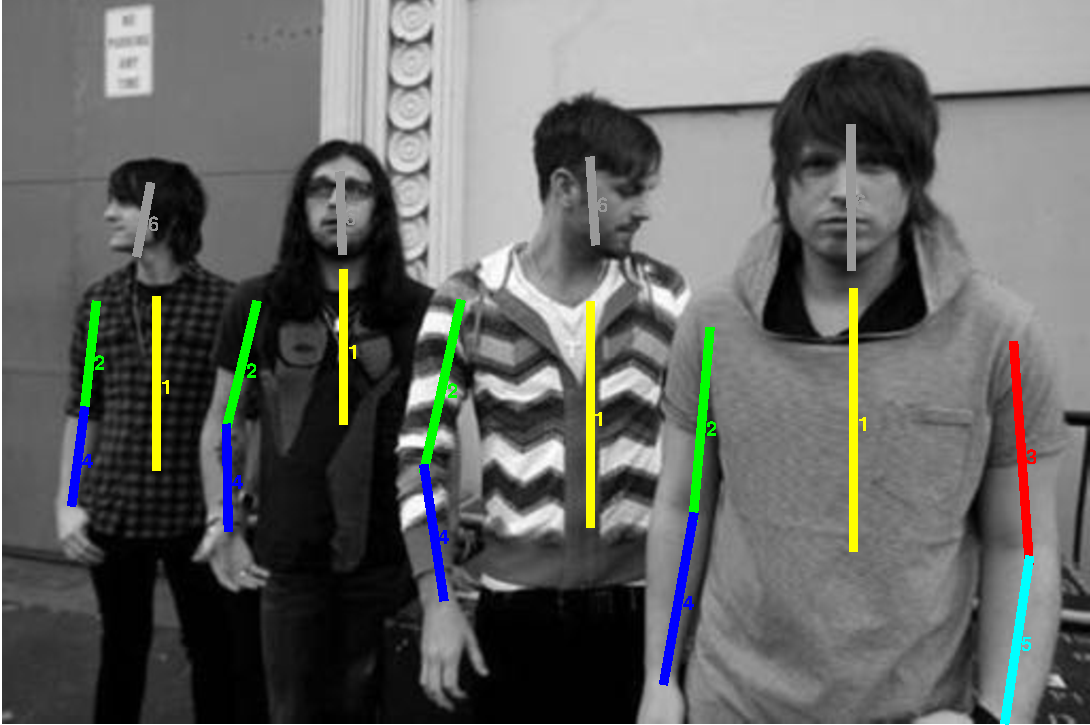
\includegraphics[height=0.145\linewidth]{imgidx_0078_sticks_waf.pdf}&
    %\includegraphics[height=0.145\linewidth]{imgidx_0020_sticks_waf.pdf}&
    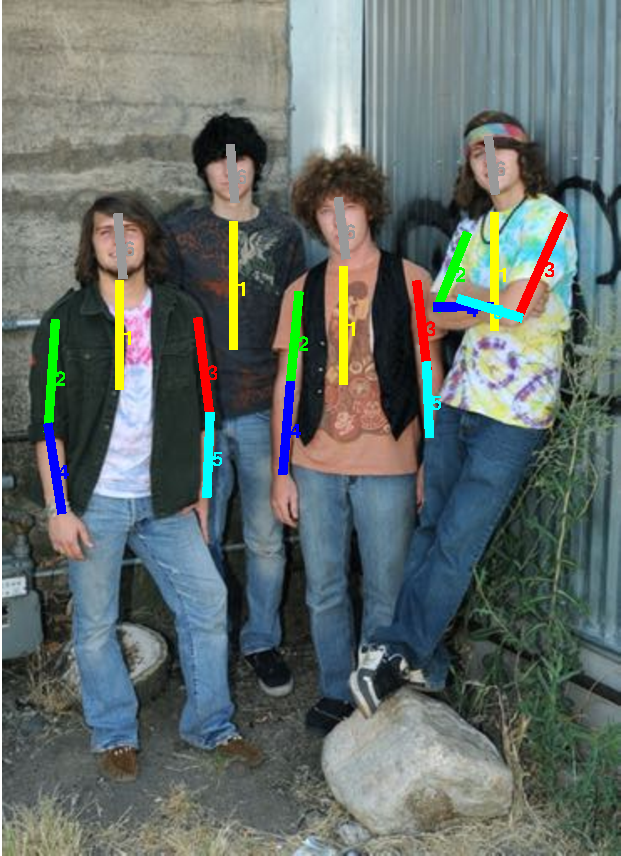
\includegraphics[height=0.145\linewidth]{imgidx_0139_sticks_waf.pdf}\\
    \begin{sideways}\bf \small Chen\&Yuille~\cite{Chen:2015:POC}\end{sideways}&
    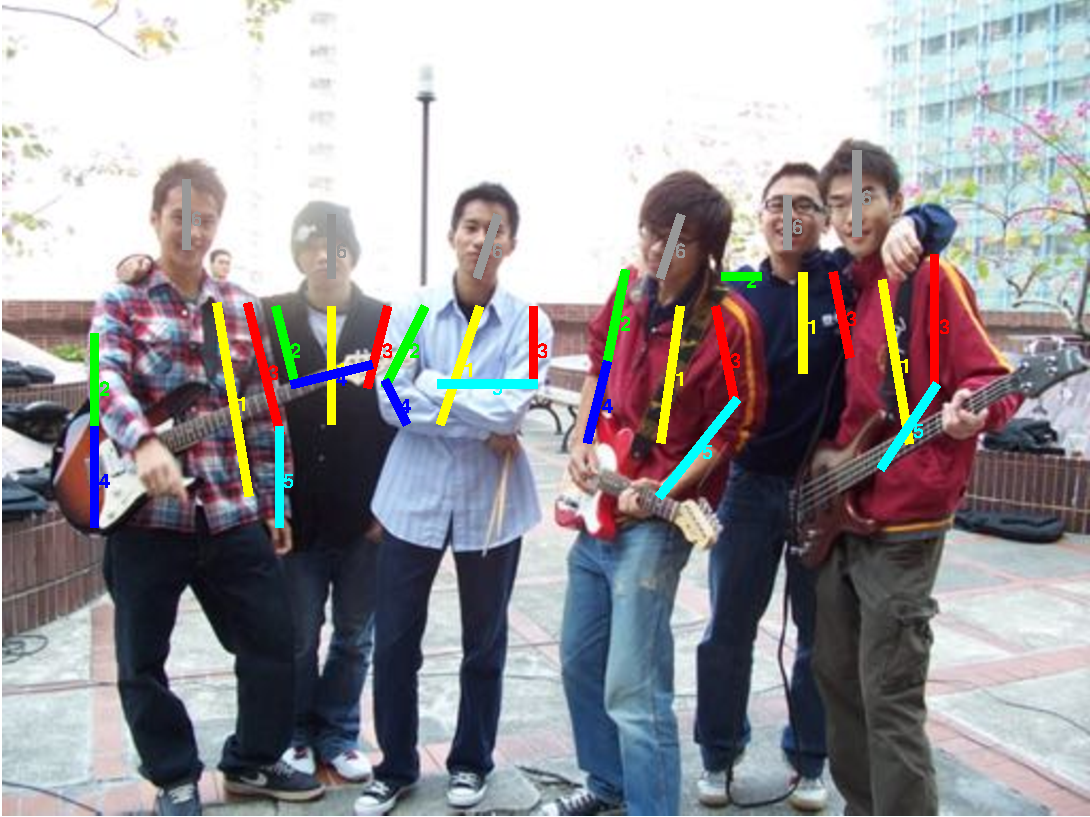
\includegraphics[height=0.145\linewidth]{imgidx_0112_sticks_chen_waf.pdf}&
    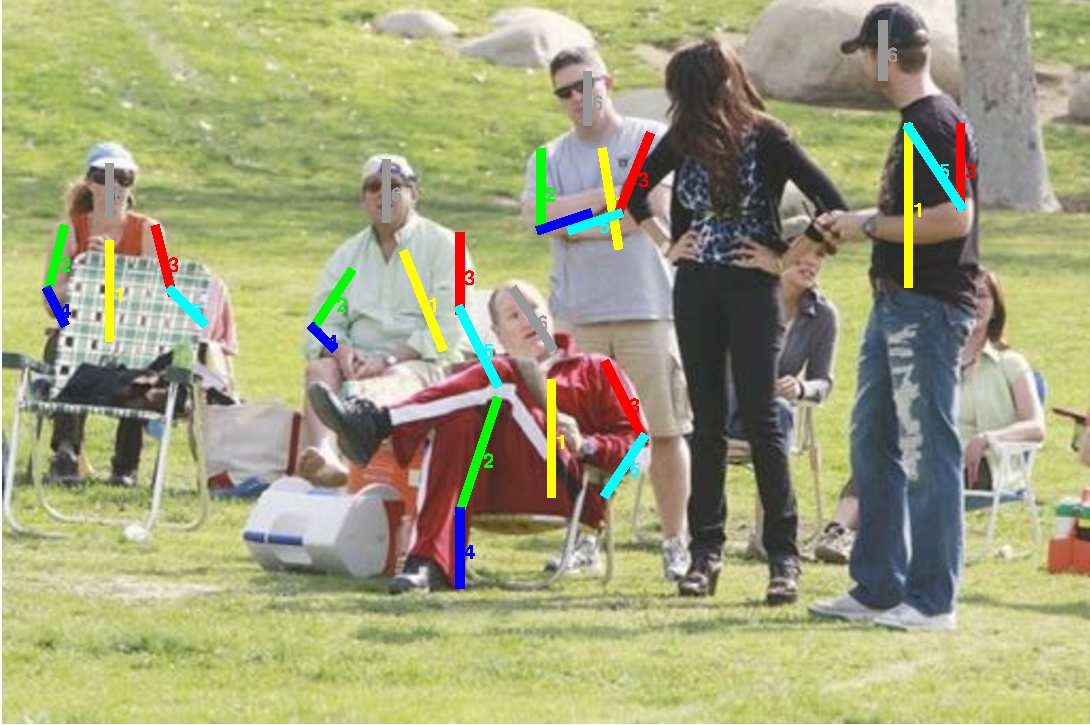
\includegraphics[height=0.145\linewidth]{imgidx_0028_sticks_chen_waf.pdf}&
    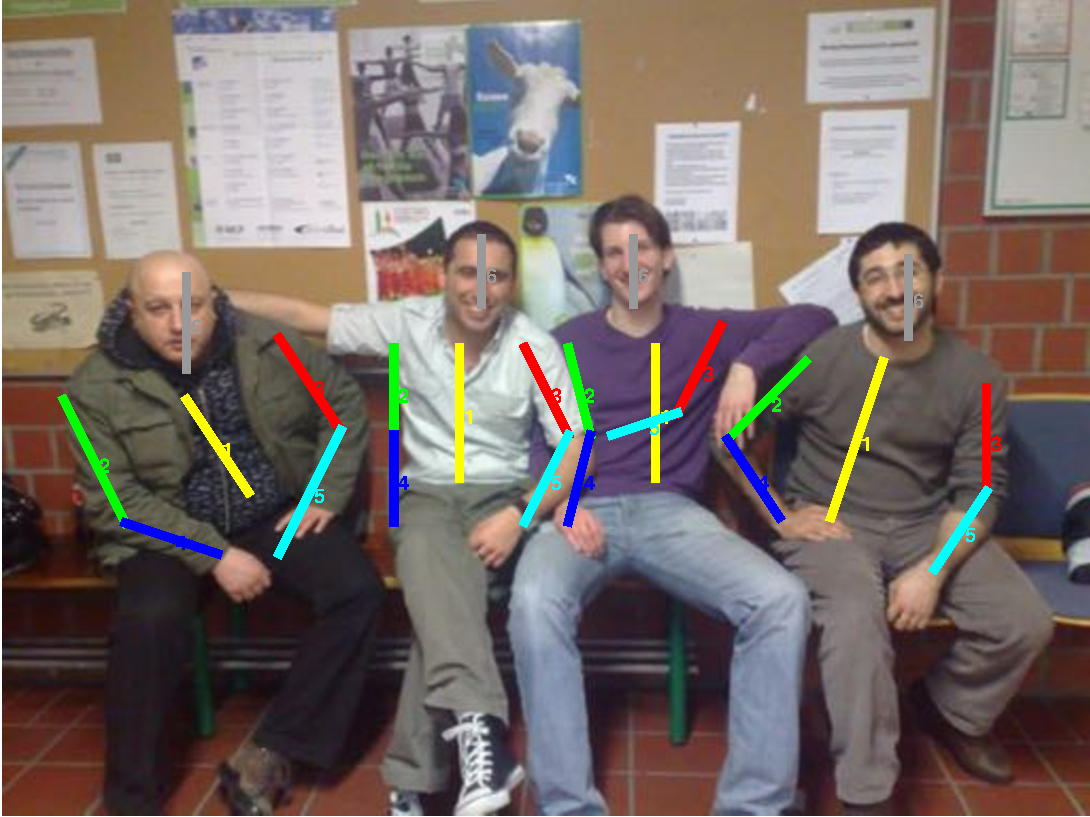
\includegraphics[height=0.145\linewidth]{imgidx_0129_sticks_chen_waf.pdf}&
    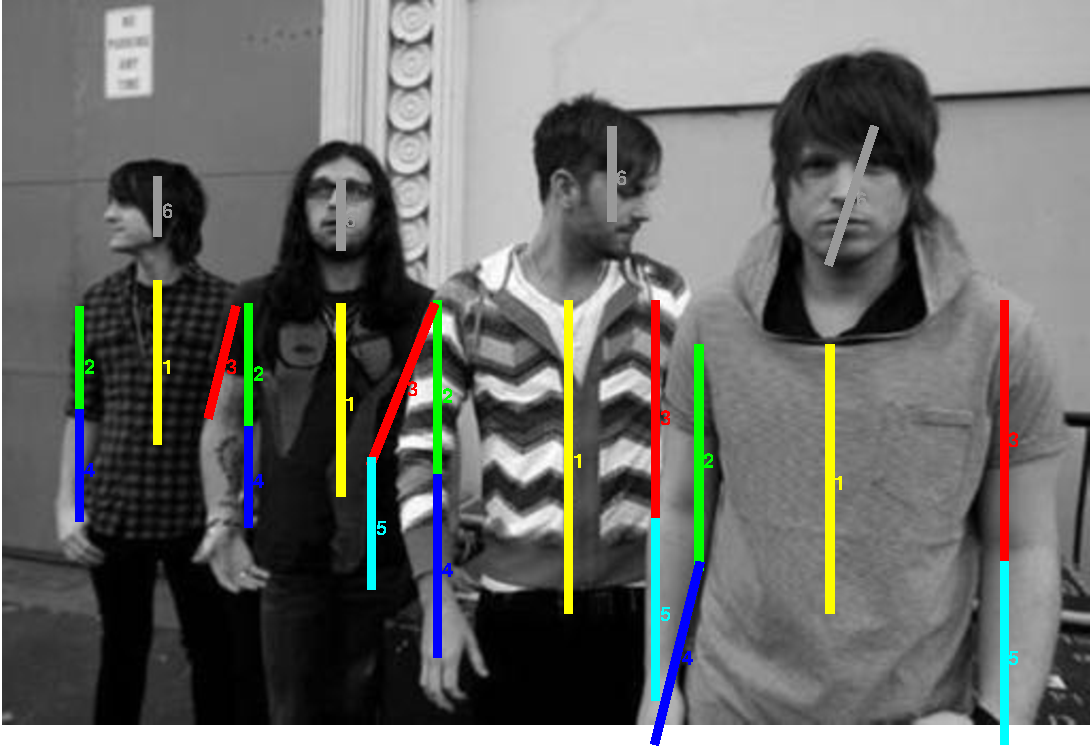
\includegraphics[height=0.145\linewidth]{imgidx_0078_sticks_chen_waf.pdf}&
    %\includegraphics[height=0.145\linewidth]{imgidx_0020_sticks_chen_waf.pdf}&
    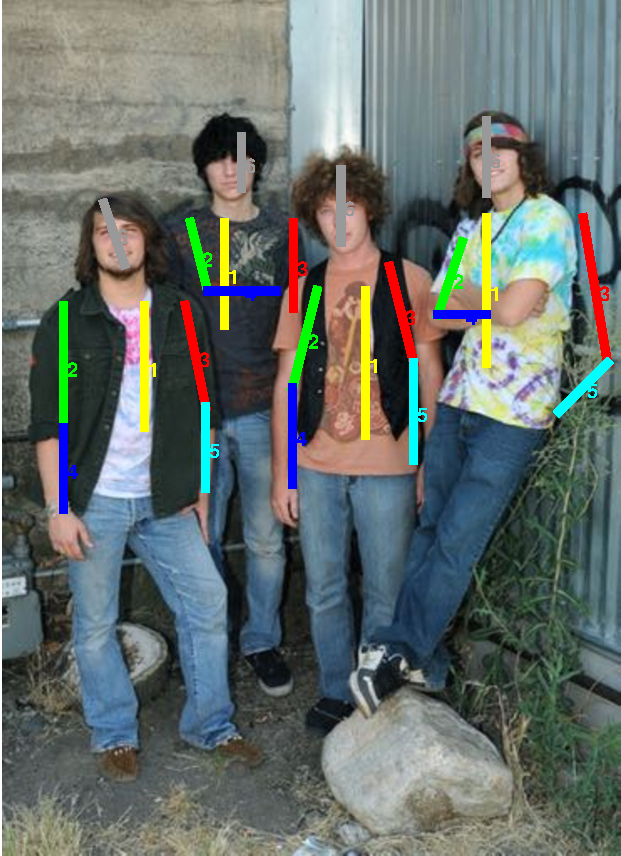
\includegraphics[height=0.145\linewidth]{imgidx_0139_sticks_chen_waf.pdf}\\
    &1&2&3&4&5\\
 %   &&&&&\\
  \end{tabular}

  \begin{tabular}{c c c c c c c}
    \begin{sideways}\bf \small\quad\quad $\detroi$\end{sideways}&
    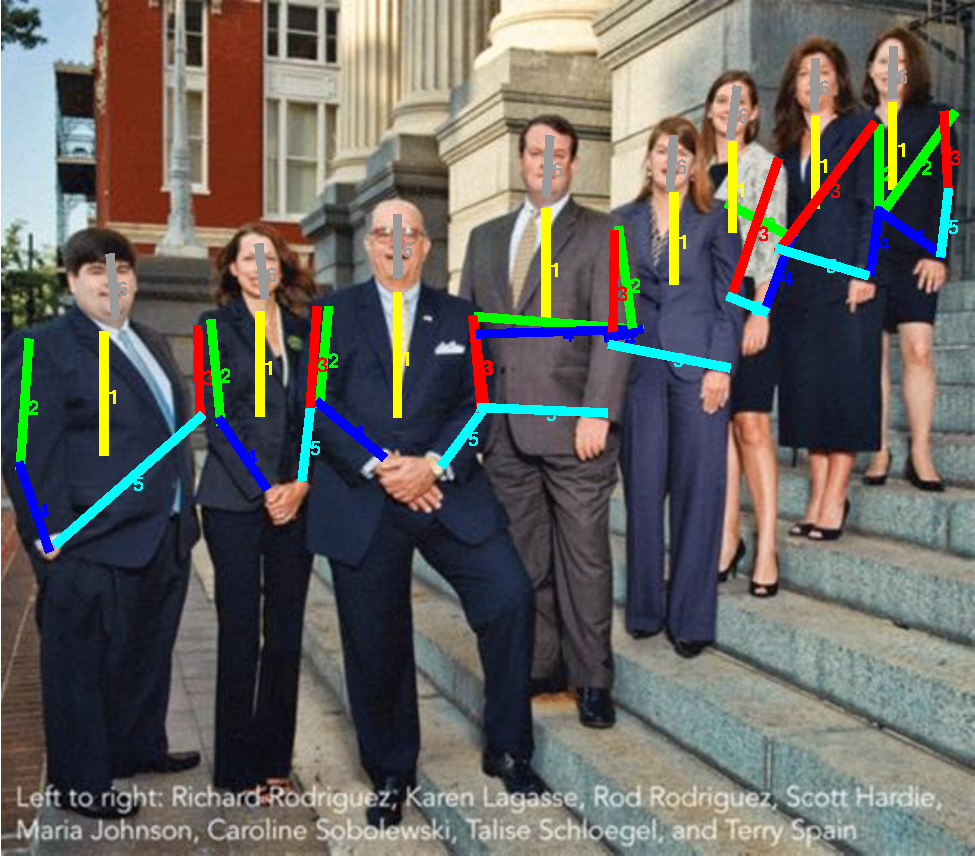
\includegraphics[height=0.145\linewidth]{imgidx_0114_sticks_unary_waf.pdf}&
    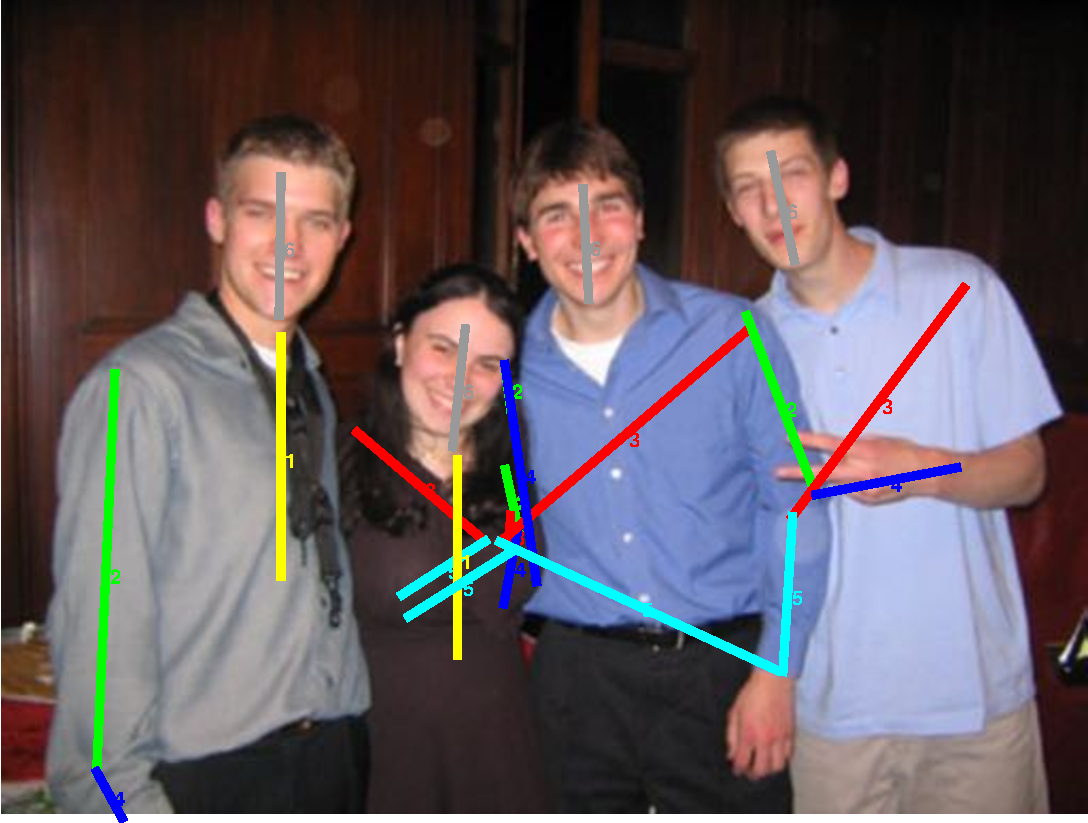
\includegraphics[height=0.145\linewidth]{imgidx_0050_sticks_unary_waf.pdf}& 
    %\includegraphics[height=0.145\linewidth]{imgidx_0069_sticks_unary_waf.pdf}& % 152
    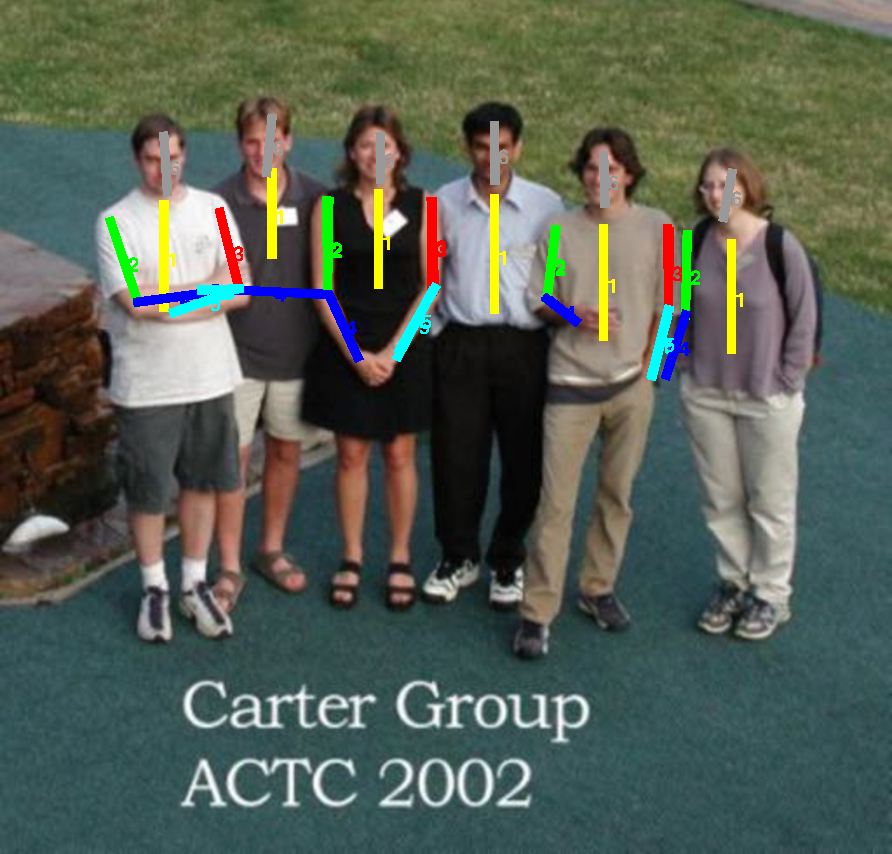
\includegraphics[height=0.145\linewidth]{imgidx_0079_sticks_unary_waf.pdf}& % 56
    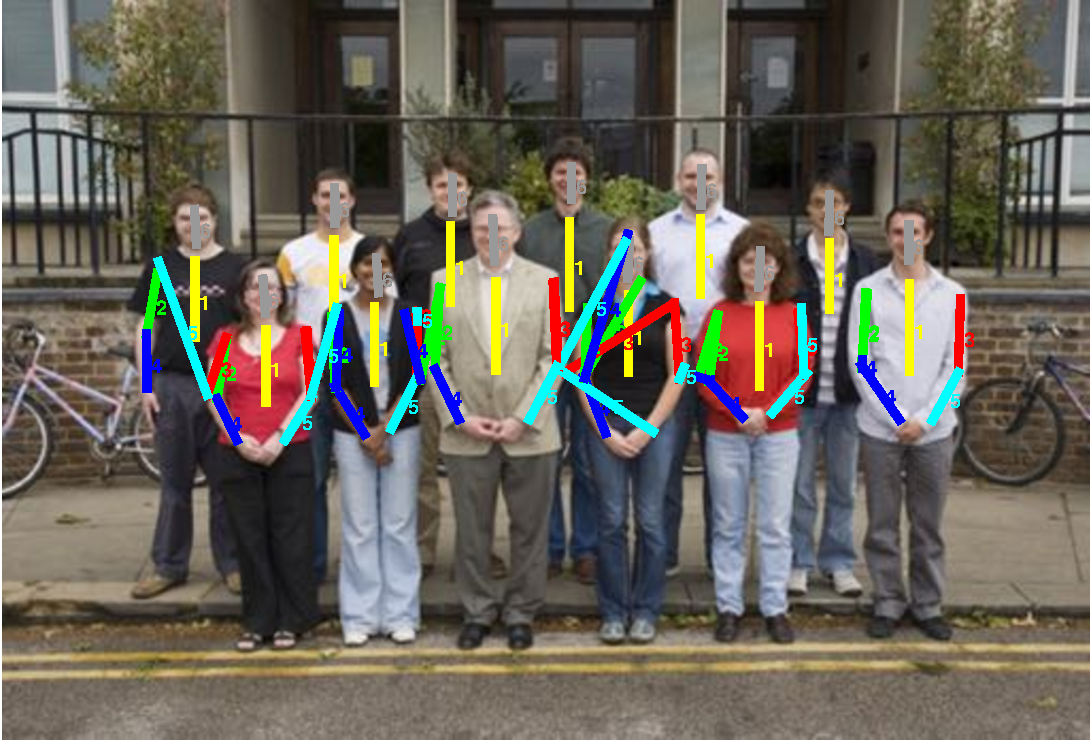
\includegraphics[height=0.145\linewidth]{imgidx_0007_sticks_unary_waf.pdf}& % 74
    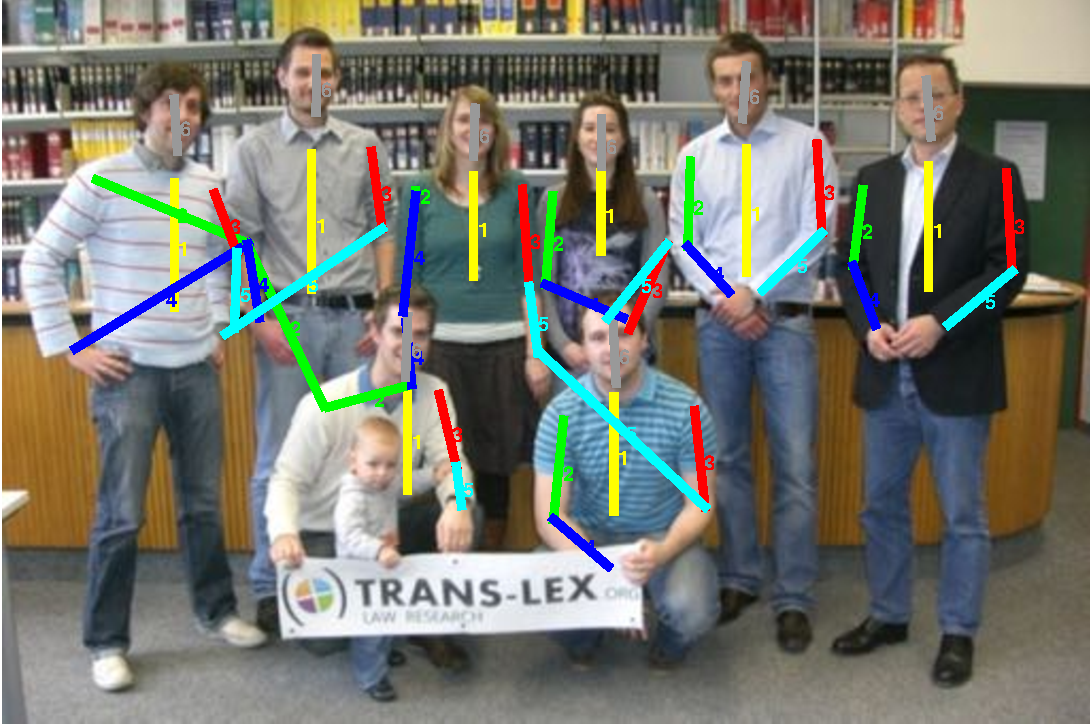
\includegraphics[height=0.145\linewidth]{imgidx_0124_sticks_unary_waf.pdf}\\
    \begin{sideways}\bf \small\quad $\deepcut~\multb$\end{sideways}&
    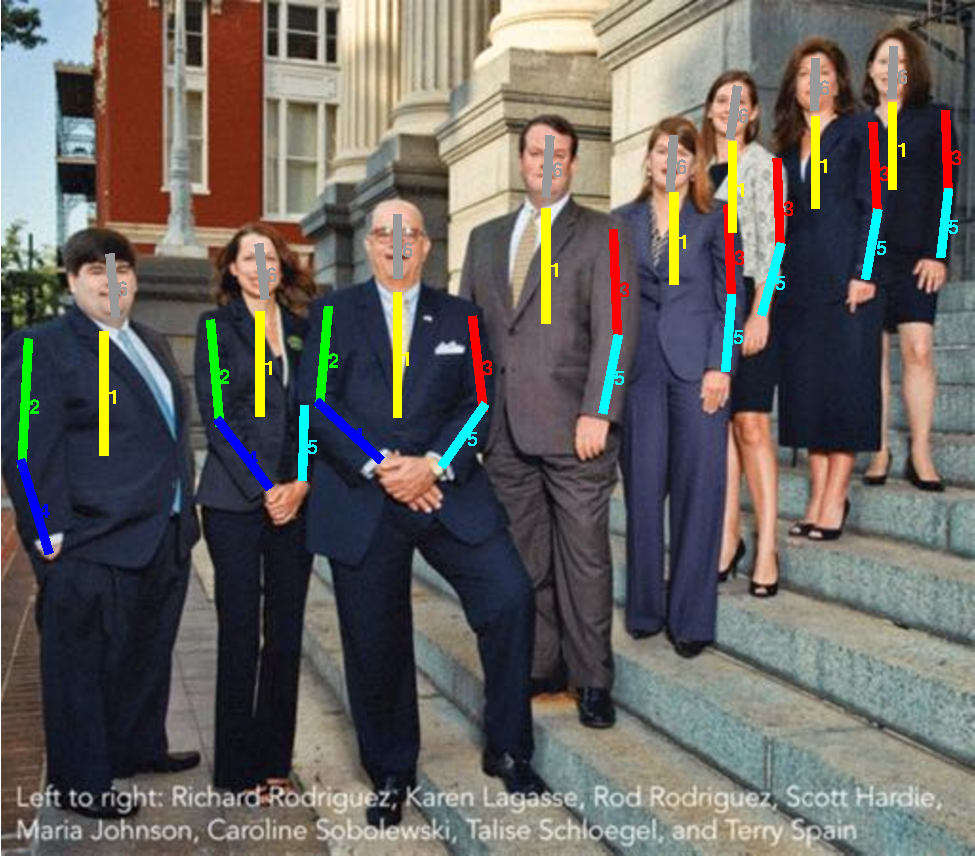
\includegraphics[height=0.145\linewidth]{imgidx_0114_sticks_waf.pdf}&
    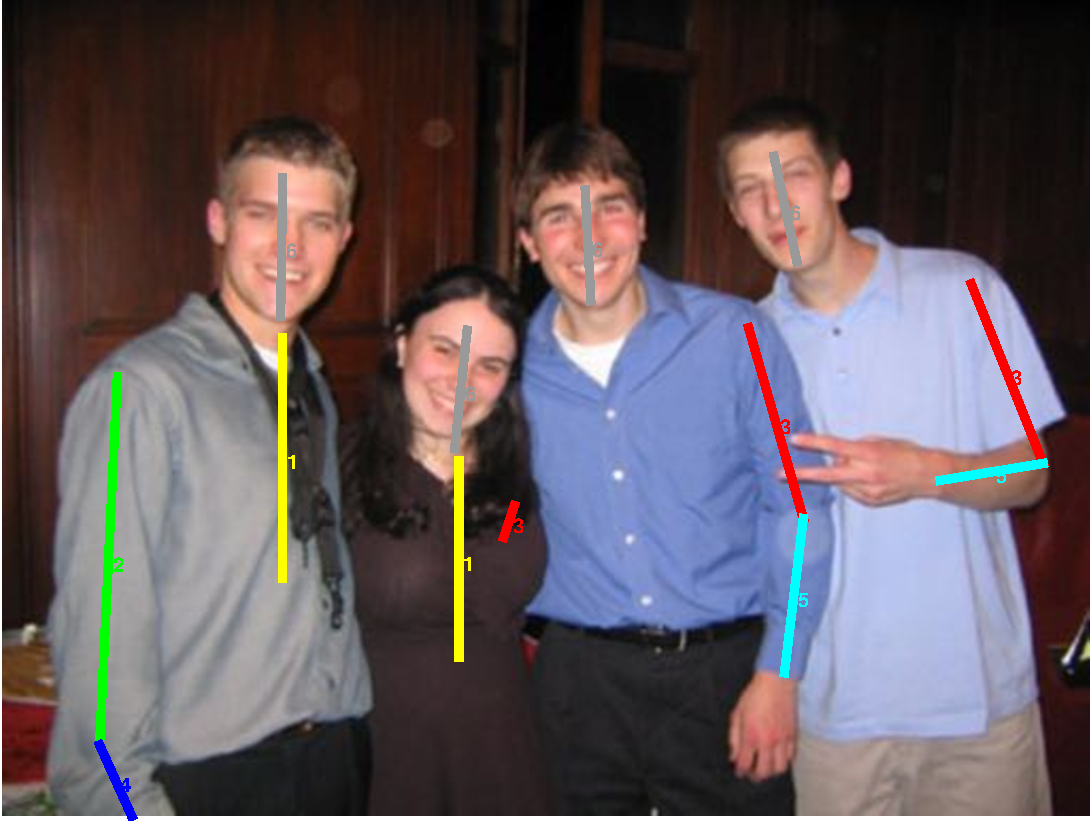
\includegraphics[height=0.145\linewidth]{imgidx_0050_sticks_waf.pdf}&
    %\includegraphics[height=0.145\linewidth]{imgidx_0069_sticks_waf.pdf}&
    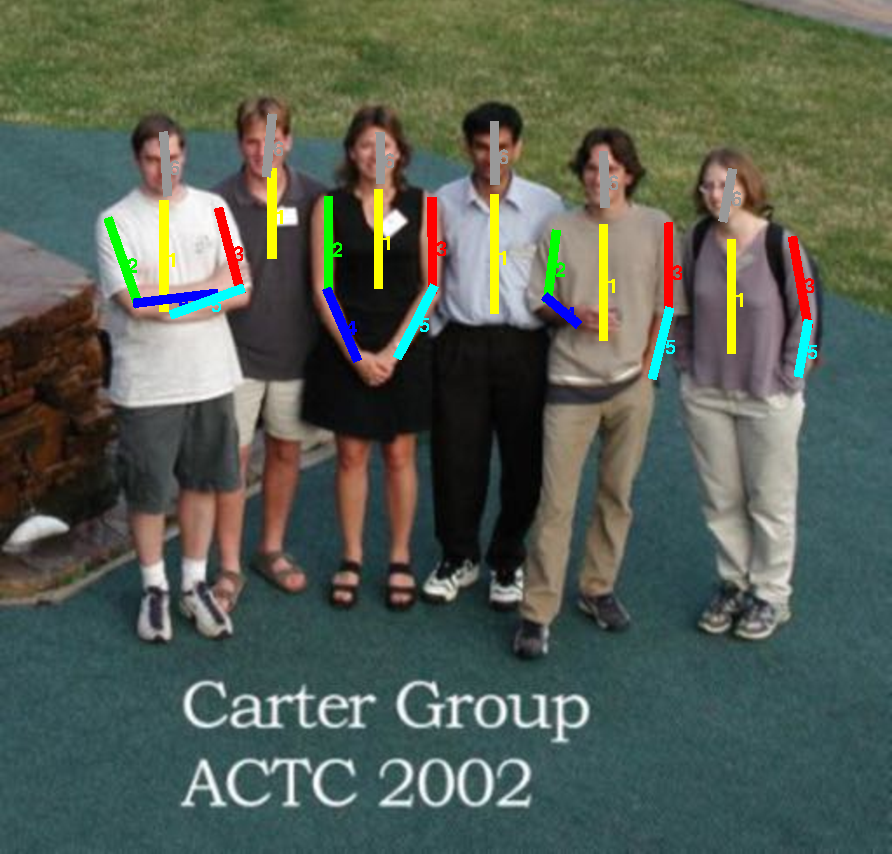
\includegraphics[height=0.145\linewidth]{imgidx_0079_sticks_waf.pdf}&
    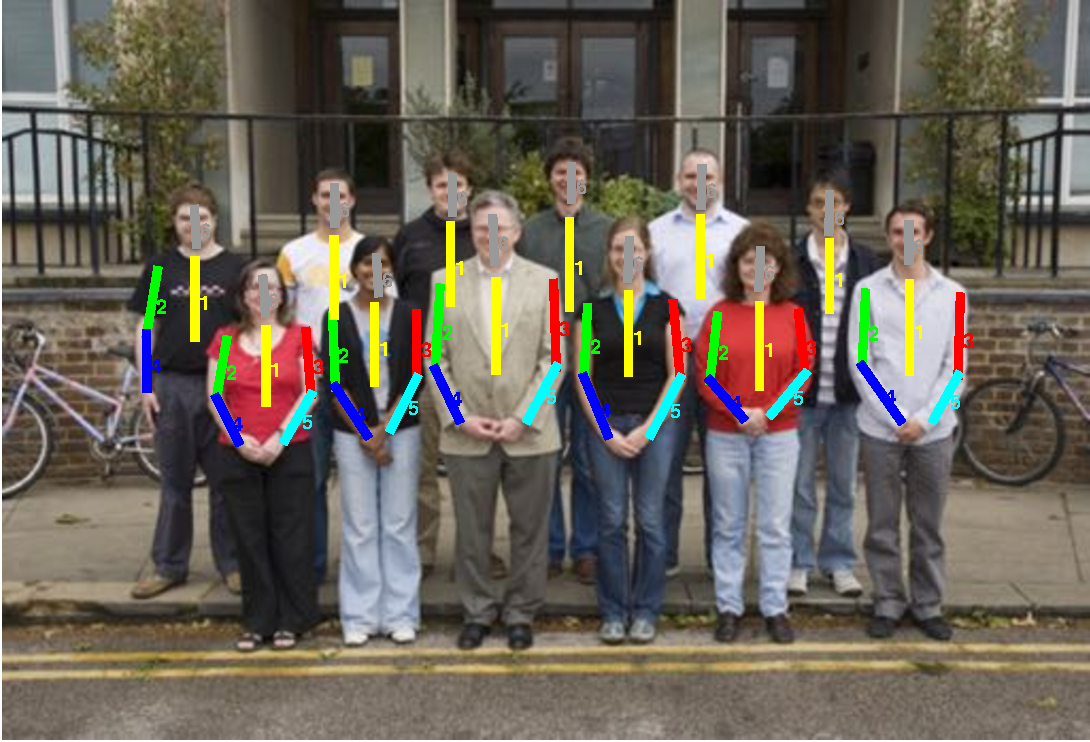
\includegraphics[height=0.145\linewidth]{imgidx_0007_sticks_waf.pdf}&
    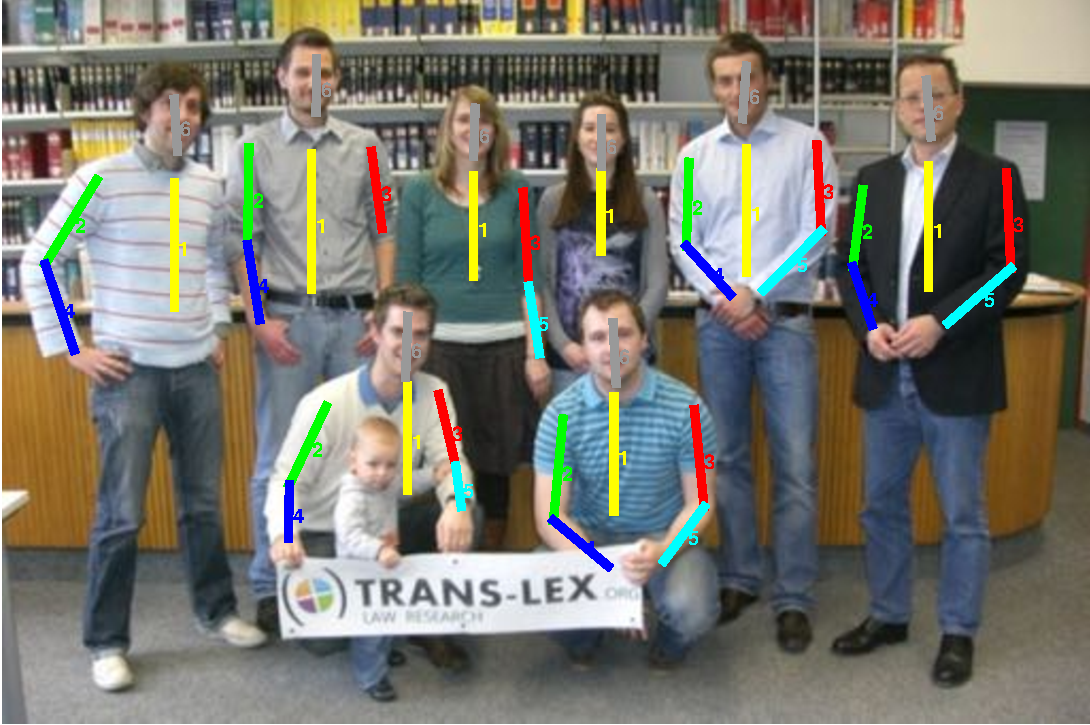
\includegraphics[height=0.145\linewidth]{imgidx_0124_sticks_waf.pdf}\\
    \begin{sideways}\bf \small Chen\&Yuille~\cite{Chen:2015:POC}\end{sideways}&
    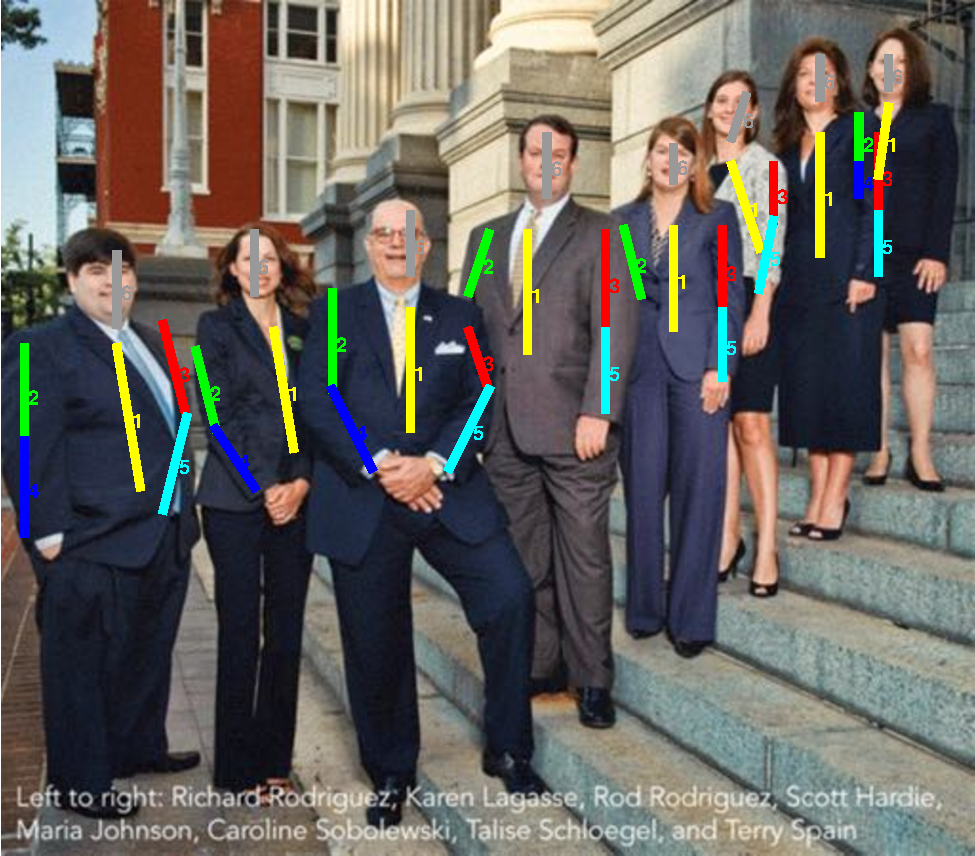
\includegraphics[height=0.145\linewidth]{imgidx_0114_sticks_chen_waf.pdf}&
    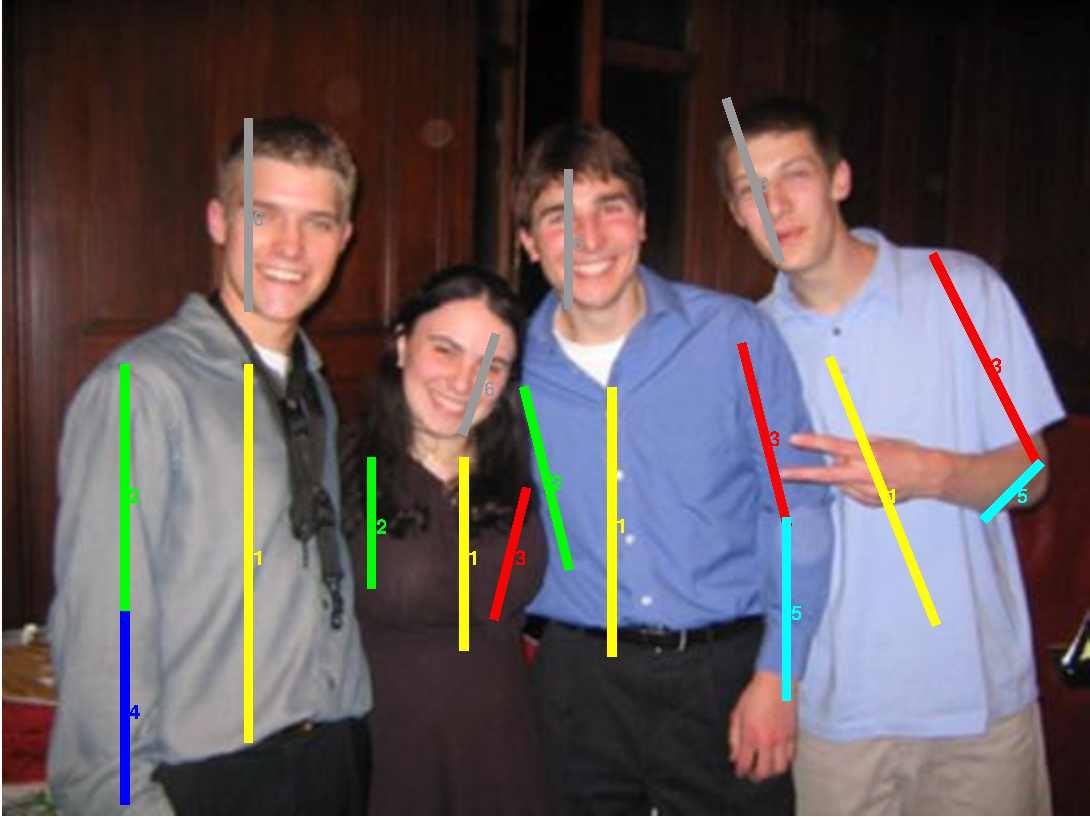
\includegraphics[height=0.145\linewidth]{imgidx_0050_sticks_chen_waf.pdf}&
    %\includegraphics[height=0.145\linewidth]{imgidx_0069_sticks_chen_waf.pdf}&
    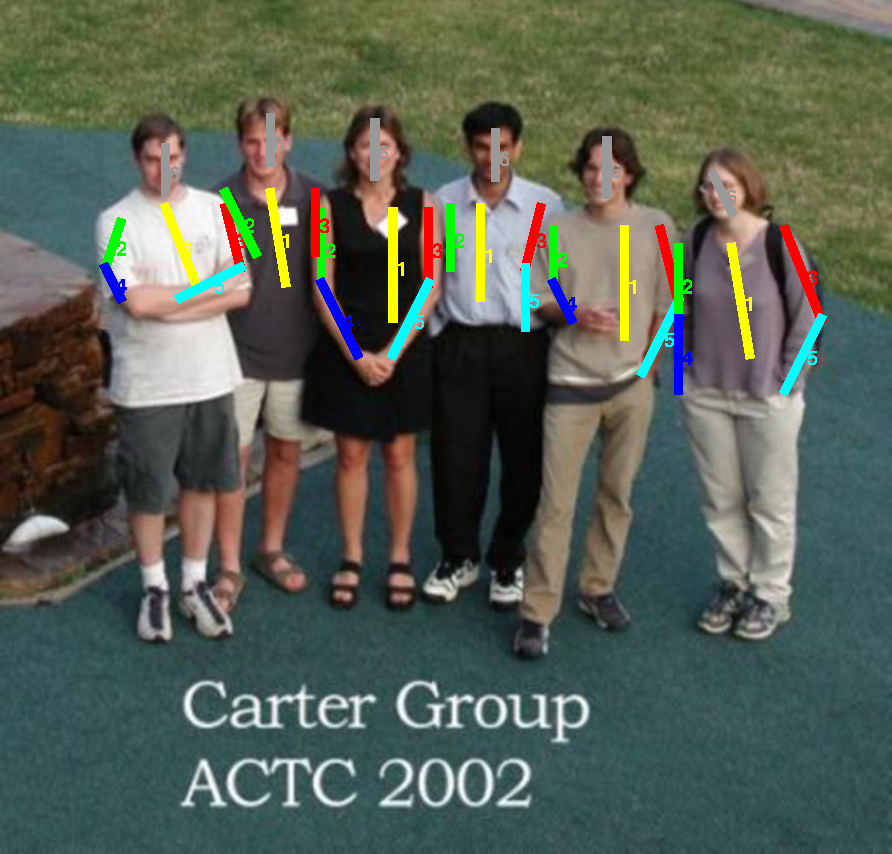
\includegraphics[height=0.145\linewidth]{imgidx_0079_sticks_chen_waf.pdf}& 
    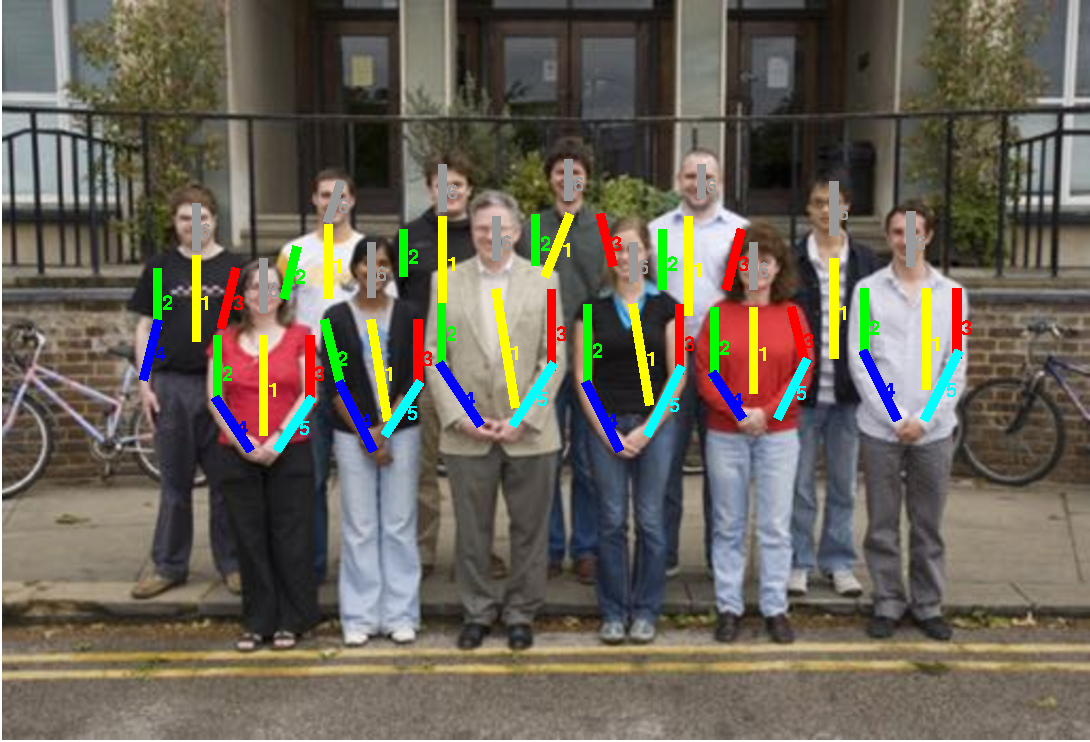
\includegraphics[height=0.145\linewidth]{imgidx_0007_sticks_chen_waf.pdf}& 
    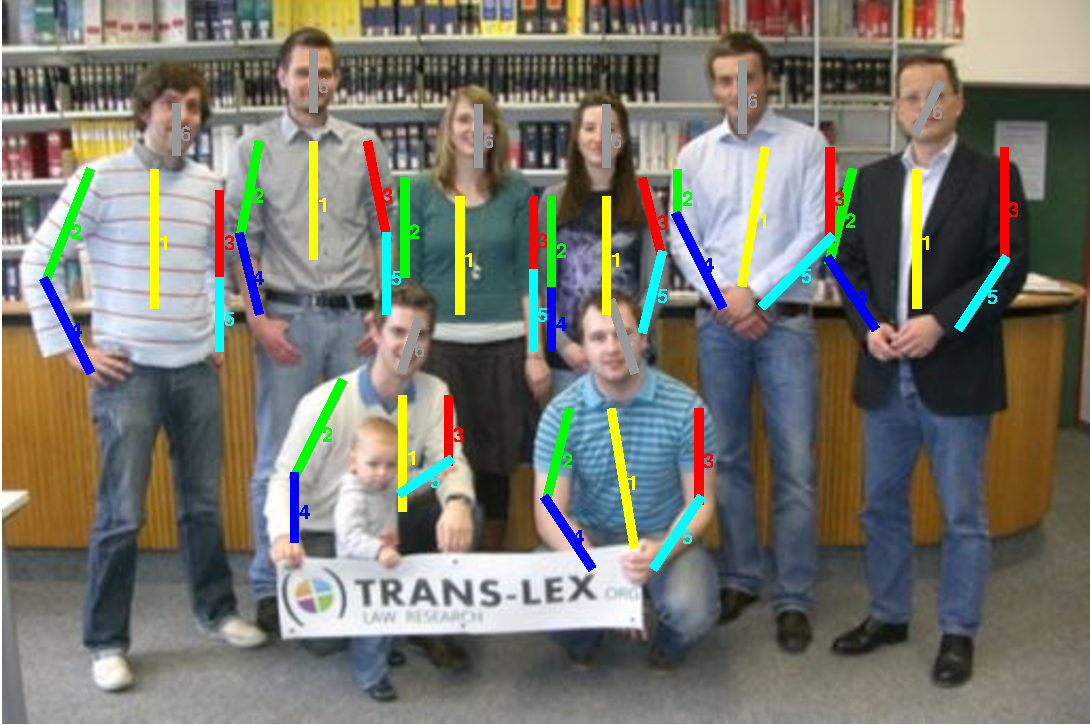
\includegraphics[height=0.145\linewidth]{imgidx_0124_sticks_chen_waf.pdf}\\
    &6&7&8&9&10\\
  \end{tabular}

%%   \begin{tabular}{c c c c c c c}
%%     \begin{sideways}\bf \small \quad\quad$\detroi$\end{sideways}&
%%     \includegraphics[height=0.145\linewidth]{imgidx_0066_sticks_unary_waf.pdf}& % 32
%%     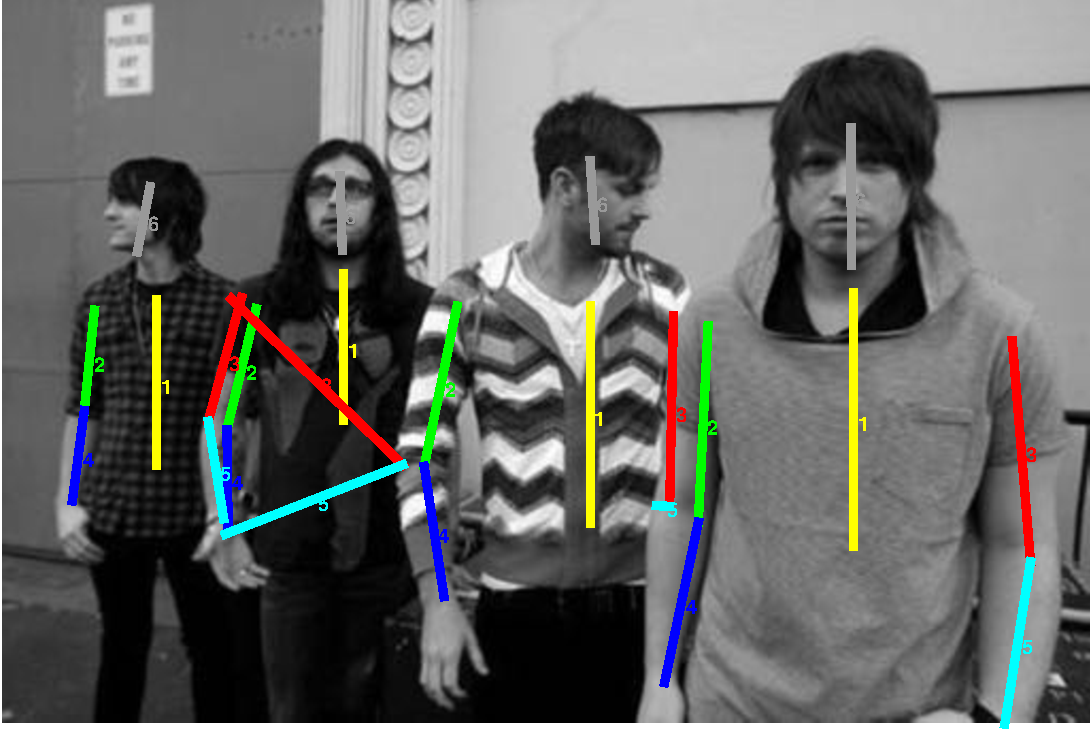
\includegraphics[height=0.145\linewidth]{imgidx_0078_sticks_unary_waf.pdf}& % 145
%%     \includegraphics[height=0.145\linewidth]{imgidx_0146_sticks_unary_waf.pdf}& 
%%     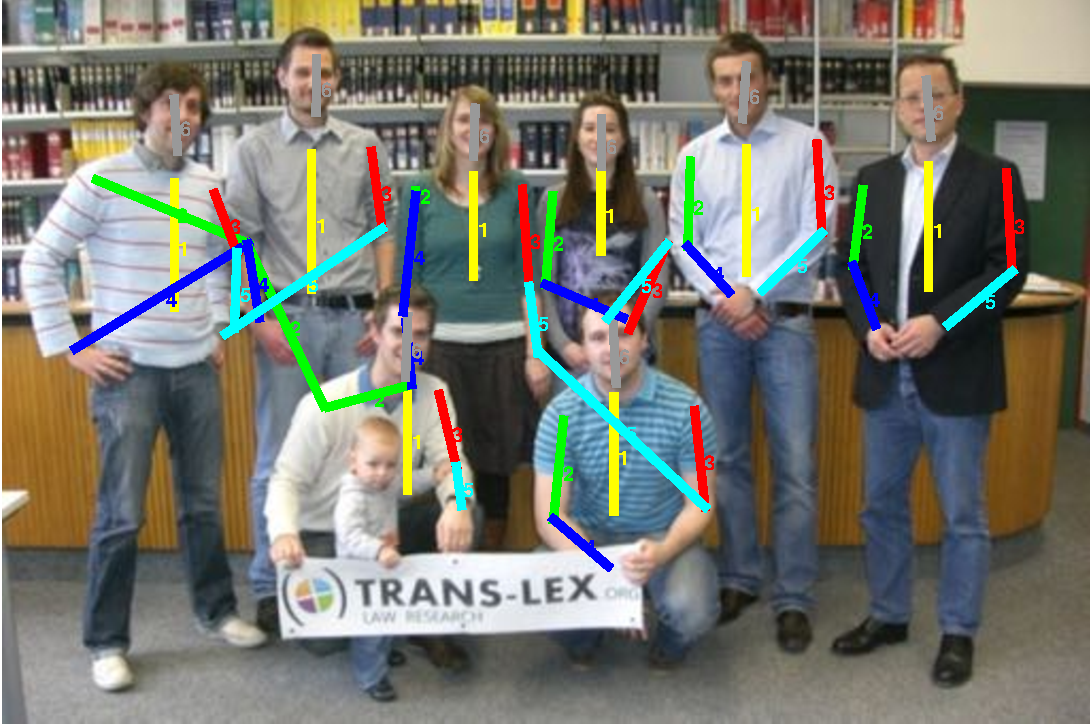
\includegraphics[height=0.145\linewidth]{imgidx_0124_sticks_unary_waf.pdf}& 
%%     \includegraphics[height=0.145\linewidth]{imgidx_0071_sticks_unary_waf.pdf}\\
%%     \begin{sideways}\bf \small \quad$\deepcut~\multb$\end{sideways}&
%%     \includegraphics[height=0.145\linewidth]{imgidx_0066_sticks_waf.pdf}&
%%     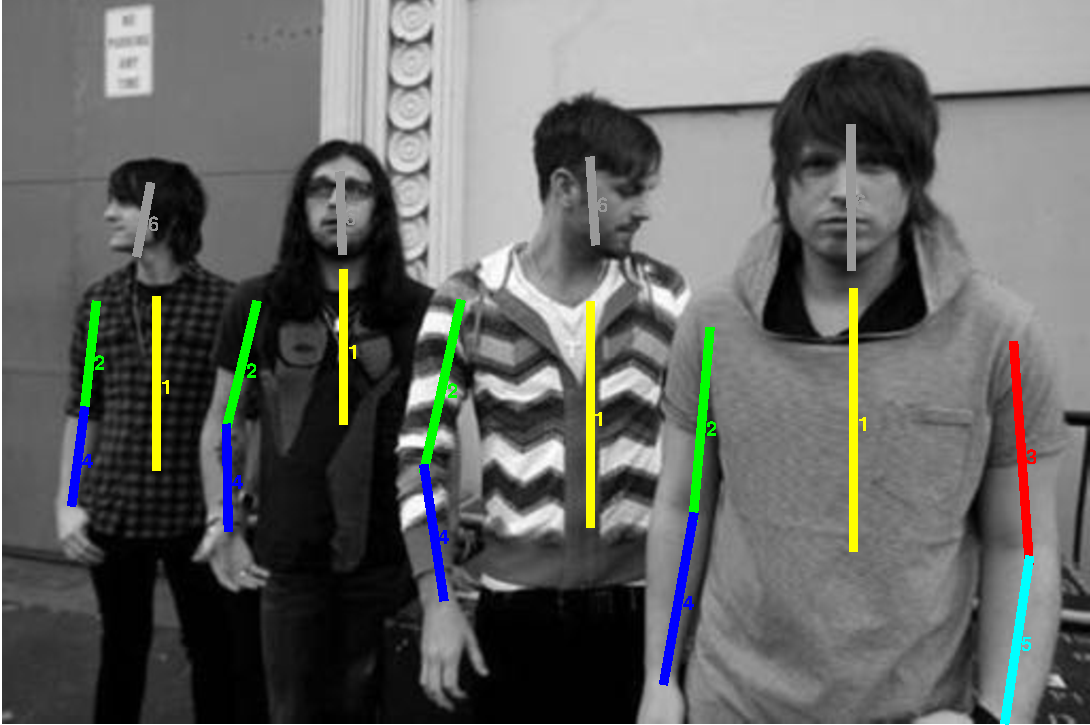
\includegraphics[height=0.145\linewidth]{imgidx_0078_sticks_waf.pdf}&
%%     \includegraphics[height=0.145\linewidth]{imgidx_0146_sticks_waf.pdf}&
%%     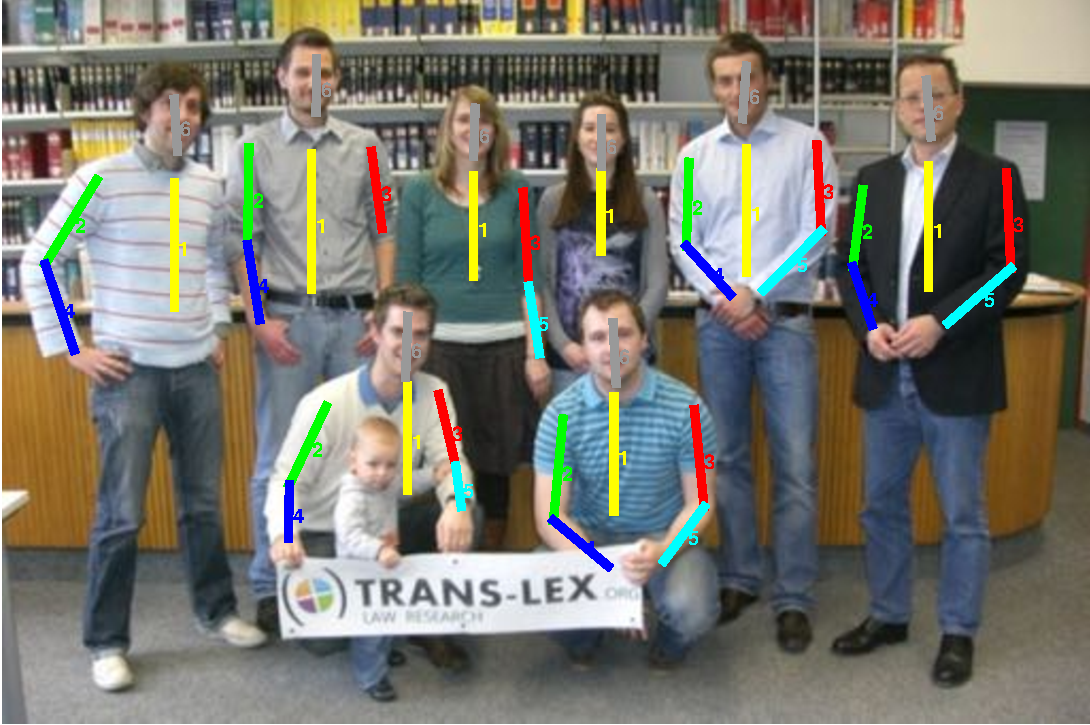
\includegraphics[height=0.145\linewidth]{imgidx_0124_sticks_waf.pdf}&
%%     \includegraphics[height=0.145\linewidth]{imgidx_0071_sticks_waf.pdf}\\
%%     \begin{sideways}\bf \small Chen\&Yuille~\cite{Chen:2015:POC}\end{sideways}&
%%     \includegraphics[height=0.145\linewidth]{imgidx_0066_sticks_chen_waf.pdf}&
%%     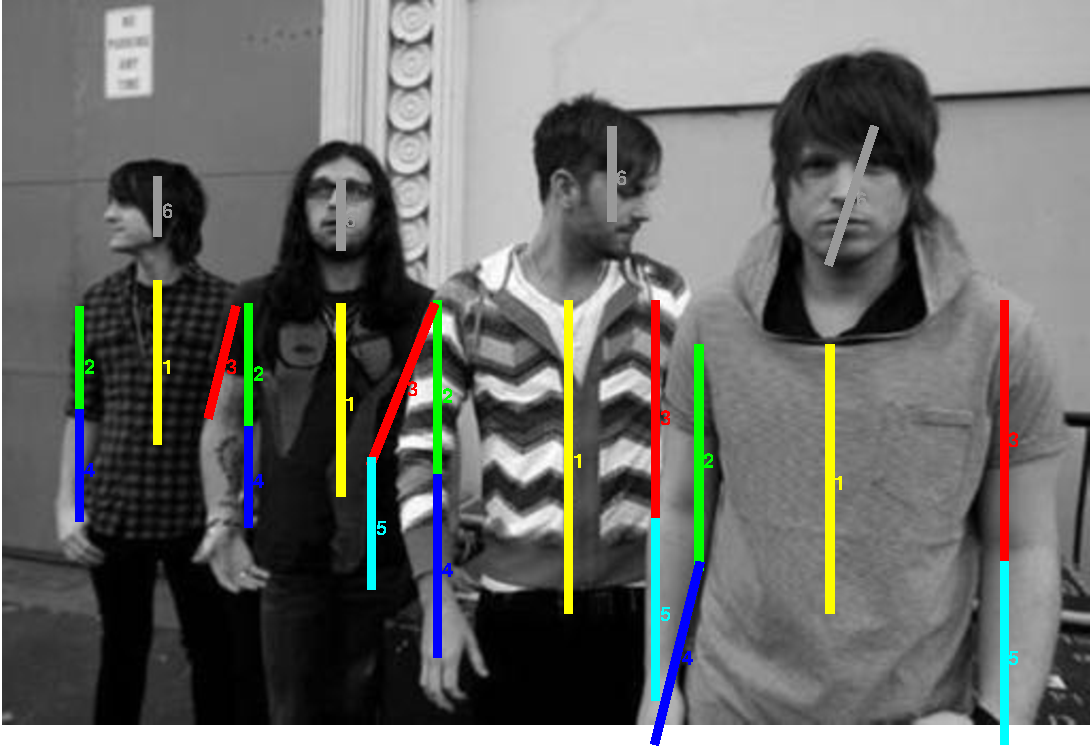
\includegraphics[height=0.145\linewidth]{imgidx_0078_sticks_chen_waf.pdf}&
%%     \includegraphics[height=0.145\linewidth]{imgidx_0146_sticks_chen_waf.pdf}&
%%     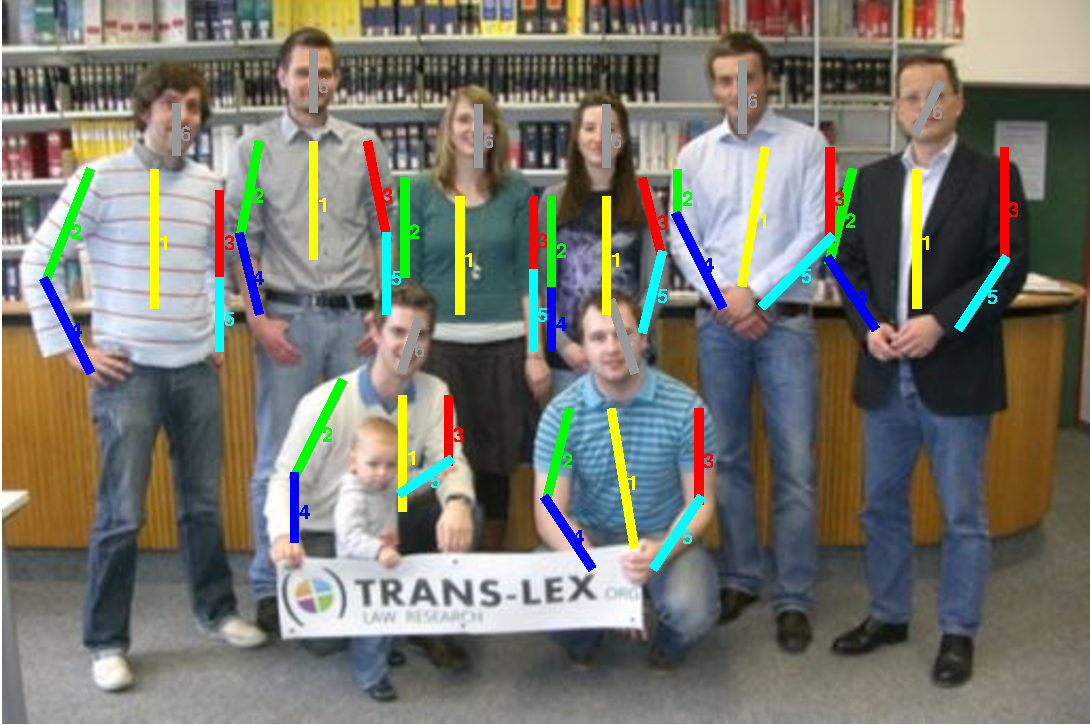
\includegraphics[height=0.145\linewidth]{imgidx_0124_sticks_chen_waf.pdf}& 
%%     \includegraphics[height=0.145\linewidth]{imgidx_0071_sticks_chen_waf.pdf}\\
%%   \end{tabular}

  %\vspace{-1.0em}
  \caption{Qualitative comparison of our joint formulation
    $\deepcut~\multb~\dense$ (rows 2, 5) to the traditional two-stage
    approach $\dense~\detroi$ (rows 1, 4) and to the approach of
    Chen\&Yuille~\cite{Chen:2015:POC} (rows 3, 6) on WAF
    dataset. $\detroi$ does not reason about occlusion and often
    predicts inconsistent body part configurations by linking the
    parts across the nearby staying people (image 4, right shoulder
    and wrist of person 2 are linked to the right elbow of person 3;
    image 5, left elbow of person 4 is linked to the left wrist of
    person 3). In contrast, $\deepcut~\multb$ predicts body part
    occlusions, disambiguates multiple and potentially overlapping
    people and correctly assembles independent detections into
    plausible body part configurations (image 4, left arms of people
    1-3 are correctly predicted to be occluded; image 5, linking of
    body parts across people 3 and 4 is corrected; image 7, occlusion
    of body parts is correctly predicted and visible parts are
    accurately estimated). In contrast to
    Chen\&Yuille~\cite{Chen:2015:POC}, $\deepcut~\multb$ better
    predicts occlusions of person's body parts by the nearby staying
    people (images 1, 3-9), but also by other objects (image 2, left
    arm of person 1 is occluded by the chair). Furthermore,
    $\deepcut~\multb$ is able to better cope with strong articulations
    and foreshortenings (image 1, person 6; image 3, person 2; image
    5, person 4; image 7, person 4; image 8, person 1). Typical
    $\deepcut~\multb$ failure case is shown in image 10: the right
    upper arm of person 3 and both arms of person 4 are not estimated
    due to missing part detection candidates.}
   %\vspace{-1.0em}
  \label{fig:qualitative_waf}
\end{figure*}

%% \begin{figure*}
%%   \centering
%%   \begin{tabular}{c c c c c c c}
%%     \begin{sideways}\bf \small\quad\quad $\detroi$\end{sideways}&
%%     \includegraphics[height=0.145\linewidth]{imgidx_0112_sticks_unary_waf.pdf}&
%%     \includegraphics[height=0.145\linewidth]{imgidx_0028_sticks_unary_waf.pdf}&
%%     \includegraphics[height=0.145\linewidth]{imgidx_0129_sticks_unary_waf.pdf}& 
%%     \includegraphics[height=0.145\linewidth]{imgidx_0058_sticks_unary_waf.pdf}& 
%%     \includegraphics[height=0.145\linewidth]{imgidx_0020_sticks_unary_waf.pdf}& % 66 
%%     \includegraphics[height=0.145\linewidth]{imgidx_0139_sticks_unary_waf.pdf}\\ 
%%     \begin{sideways}\bf \small\quad $\deepcut~\multb$\end{sideways}&
%%     \includegraphics[height=0.145\linewidth]{imgidx_0112_sticks_waf.pdf}&
%%     \includegraphics[height=0.145\linewidth]{imgidx_0028_sticks_waf.pdf}&
%%     \includegraphics[height=0.145\linewidth]{imgidx_0129_sticks_waf.pdf}&
%%     \includegraphics[height=0.145\linewidth]{imgidx_0058_sticks_waf.pdf}&
%%     \includegraphics[height=0.145\linewidth]{imgidx_0020_sticks_waf.pdf}&
%%     \includegraphics[height=0.145\linewidth]{imgidx_0139_sticks_waf.pdf}\\
%%     \begin{sideways}\bf \small Chen\&Yuille~\cite{Chen:2015:POC}\end{sideways}&
%%     \includegraphics[height=0.145\linewidth]{imgidx_0112_sticks_chen_waf.pdf}&
%%     \includegraphics[height=0.145\linewidth]{imgidx_0028_sticks_chen_waf.pdf}&
%%     \includegraphics[height=0.145\linewidth]{imgidx_0129_sticks_chen_waf.pdf}&
%%     \includegraphics[height=0.145\linewidth]{imgidx_0058_sticks_chen_waf.pdf}&
%%     \includegraphics[height=0.145\linewidth]{imgidx_0020_sticks_chen_waf.pdf}&
%%     \includegraphics[height=0.145\linewidth]{imgidx_0139_sticks_chen_waf.pdf}\\
%%   \end{tabular}

%%   \begin{tabular}{c c c c c c c}
%%     \begin{sideways}\bf \small\quad\quad $\detroi$\end{sideways}&
%%     \includegraphics[height=0.145\linewidth]{imgidx_0114_sticks_unary_waf.pdf}&
%%     \includegraphics[height=0.145\linewidth]{imgidx_0050_sticks_unary_waf.pdf}& 
%%     \includegraphics[height=0.145\linewidth]{imgidx_0069_sticks_unary_waf.pdf}& % 152
%%     \includegraphics[height=0.145\linewidth]{imgidx_0079_sticks_unary_waf.pdf}& % 56
%%     \includegraphics[height=0.145\linewidth]{imgidx_0074_sticks_unary_waf.pdf}& % 66 
%%     \includegraphics[height=0.145\linewidth]{imgidx_0007_sticks_unary_waf.pdf}\\
%%     \begin{sideways}\bf \small\quad $\deepcut~\multb$\end{sideways}&
%%     \includegraphics[height=0.145\linewidth]{imgidx_0114_sticks_waf.pdf}&
%%     \includegraphics[height=0.145\linewidth]{imgidx_0050_sticks_waf.pdf}&
%%     \includegraphics[height=0.145\linewidth]{imgidx_0069_sticks_waf.pdf}&
%%     \includegraphics[height=0.145\linewidth]{imgidx_0079_sticks_waf.pdf}&
%%     \includegraphics[height=0.145\linewidth]{imgidx_0074_sticks_waf.pdf}&
%%     \includegraphics[height=0.145\linewidth]{imgidx_0007_sticks_waf.pdf}\\
%%     \begin{sideways}\bf \small Chen\&Yuille~\cite{Chen:2015:POC}\end{sideways}&
%%     \includegraphics[height=0.145\linewidth]{imgidx_0114_sticks_chen_waf.pdf}&
%%     \includegraphics[height=0.145\linewidth]{imgidx_0050_sticks_chen_waf.pdf}&
%%     \includegraphics[height=0.145\linewidth]{imgidx_0069_sticks_chen_waf.pdf}&
%%     \includegraphics[height=0.145\linewidth]{imgidx_0079_sticks_chen_waf.pdf}& 
%%     \includegraphics[height=0.145\linewidth]{imgidx_0074_sticks_chen_waf.pdf}& 
%%     \includegraphics[height=0.145\linewidth]{imgidx_0007_sticks_chen_waf.pdf}\\
%%   \end{tabular}

%%   \begin{tabular}{c c c c c c c}
%%     \begin{sideways}\bf \small \quad\quad$\detroi$\end{sideways}&
%%     \includegraphics[height=0.145\linewidth]{imgidx_0066_sticks_unary_waf.pdf}& % 32
%%     \includegraphics[height=0.145\linewidth]{imgidx_0078_sticks_unary_waf.pdf}& % 145
%%     \includegraphics[height=0.145\linewidth]{imgidx_0146_sticks_unary_waf.pdf}& 
%%     \includegraphics[height=0.145\linewidth]{imgidx_0124_sticks_unary_waf.pdf}& 
%%     \includegraphics[height=0.145\linewidth]{imgidx_0071_sticks_unary_waf.pdf}\\
%%     \begin{sideways}\bf \small \quad$\deepcut~\multb$\end{sideways}&
%%     \includegraphics[height=0.145\linewidth]{imgidx_0066_sticks_waf.pdf}&
%%     \includegraphics[height=0.145\linewidth]{imgidx_0078_sticks_waf.pdf}&
%%     \includegraphics[height=0.145\linewidth]{imgidx_0146_sticks_waf.pdf}&
%%     \includegraphics[height=0.145\linewidth]{imgidx_0124_sticks_waf.pdf}&
%%     \includegraphics[height=0.145\linewidth]{imgidx_0071_sticks_waf.pdf}\\
%%     \begin{sideways}\bf \small Chen\&Yuille~\cite{Chen:2015:POC}\end{sideways}&
%%     \includegraphics[height=0.145\linewidth]{imgidx_0066_sticks_chen_waf.pdf}&
%%     \includegraphics[height=0.145\linewidth]{imgidx_0078_sticks_chen_waf.pdf}&
%%     \includegraphics[height=0.145\linewidth]{imgidx_0146_sticks_chen_waf.pdf}&
%%     \includegraphics[height=0.145\linewidth]{imgidx_0124_sticks_chen_waf.pdf}& 
%%     \includegraphics[height=0.145\linewidth]{imgidx_0071_sticks_chen_waf.pdf}\\
%%   \end{tabular}

%%   %\vspace{-0.1em}
%%   \caption{Qualitative comparison of our joint formulation
%%     ($\deepcut~\multb~\dense$ - middle) to the traditional two-stage
%%     approach ($\dense~\detroi$ - top) and to the approach of
%%     Chen\&Yuille~\cite{Chen:2015:POC} (bottom) on WAF dataset.}
%%    \vspace{-1.0em}
%%   \label{fig:qualitative_waf}
%% \end{figure*}
